\lhead{\emph{Overview of Magnetic Field Systems}}
\chapter{Overview of Magnetic Field Systems}\label{ch:magnetics}

% \begin{itemize}
%     \item Literature Review
%     \item Literature Review of nEDM Experiments
%     \item Literature Review of Current Approaches to Magnetic Field
%     \item Magnetic Environment at TRIUMF
%     \item Magnetic Requirements for TRIUMF
%     \item Design Concepts for TRIUMF
% \end{itemize}


This chapter describes the magnetic field requirement for the TUCAN nEDM experiment. The magnetic subsystems which are required to to achieve the magnetic field requirement are introduced. I have also briefly reviewed the current status worldwide of the use of active magnetic shielding for nEDM measurements.
% Finally, the chapter ends with  describing the main objective for this thesis. 


\section{Magnetic Field Requirements for TUCAN nEDM Experiment}\label{sec:msr}

The magnetic field requirements to achieve $10^{-27}$~e$\cdot$cm sensitivity level for TUCAN nEDM experiment are :

\begin{itemize}

    \item The experimental magnetic field $B_0\sim1~\mu$T, 
    \item The magnetic stability upper limit on $B_0\sim1$~pT {\it i.e.} $<$~pT drift in one nEDM measurement cycle, and 
    \item The magnetic homogeneity upper limit on $B_0\sim1$~nT/m {\it i.e.} $<$~nT/m field gradient. 
    
\end{itemize}





% To achieve $10^{-27}$ e$\cdot$cm sensitivity level for TUCAN nEDM experiment, it must be ensured to have a magnetic field of $\sim$1 pT stability i.e. $<$pT drift in one nEDM measurement cycle and $\sim$1 nT/m homogeneity. So, the magnetic field should be precisely monitored and controlled which imply that the coil generating the field must be better than that level. The nEDM experiment itself along with passive shielding will be under a Magnetically Shielded Room (MSR) and around which compensation coils will be placed for active shielding which needs to be designed as shown in Fig. \ref{fig:msr}. 
% A stable and homogeneous magnetic field $\bm{B_o}$ ($\sim$1 $\mu$T) is required to achieve the desired $10^{-27}$ e$\cdot$cm sensitivity level for TUCAN nEDM experiment. \\

A particularly challenging aspect is that the TUCAN nEDM experiment will be located in the fringe field of TRIUMF cyclotron. At the location of the experiment, the fringe could be as large as $7-8$ times the magnetic field of the earth ($\sim376~\mu$T) with $\sim100~\mu$T/m gradients~\cite{sarte}. Furthermore, large changes due to external magnetic sources are possible. These sources include nearby beam line magnets or the movement of large magnetic objects such as the 50-ton crane in Meson Hall. In general, the cyclotron field is very stable. During quiet times  $\sim100$~nT fluctuations are observed which are consistent in scale with typical drifts in Earth's magnetic field and typical laboratory environments. But the fluctuations during the day could be e.g. as large as  $\sim16~\mu$T due to movement of the 50-ton crane based on measurements done in 2012. The magnetic field information will be quantified in near future with new fluxgates which are being set up in the Meson Hall~\cite{beapriv}.


% \fig{Images/msr_pic2}{width = 0.6\textwidth}{Schematic diagram for the TUCAN nEDM magnetics. From outside in: The active compensation system which is just outside the magnetically shielded room (MSR) will decrease $\Delta B\sim\rm{10^2}$ times. The four passive shielding layers of MSR will decrease $\Delta B\sim\rm{10^6}$ times. Internal to the innermost shielding layer, there is internal coil system ($\bm{B_0}$ and $\bm{B_1}$ coils) to generate the magnetic fields for the Ramsey cycle followed by the UCN and the co-magnetometers. \label{fig:msr}}{Schematic diagram for the TUCAN nEDM magnetics}
\fig{Images/msr_pic3}{width = 0.6\textwidth}{Schematic diagram for the TUCAN nEDM magnetic field systems. From outside in: The active compensation system external to the magnetically shielded room (MSR). Internal to the innermost of the four passive shielding layers of MSR, there is internal coil system ($B_0$ and $B_1$ coils) followed by the alkaline magnetometers, UCN, and the comagnetometers. \label{fig:msr}}{Schematic diagram for the TUCAN nEDM magnetic field systems}





% We need several complimentary approaches actively and passively to shield the experimental volume from the external fields. As well to stabilize and monitor the applied experimental fields. The nEDM experiment itself along with passive shielding will be under a Magnetically Shielded Room (MSR) and around which compensation coils will be placed for active shielding which needs to be designed. The general approach is shown in Fig.~\ref{fig:msr} and each element is discussed in further detail below. 
We need several approaches combining active and passive magnetic shielding in order to insulate the experimental volume from the extraneous magnetic fields. There are also several techniques used to generate, stabilize and monitor the applied experimental fields. 

% The nEDM experiment itself along with passive shielding will be under a Magnetically Shielded Room (MSR) and around which compensation coils will be placed for active shielding which needs to be designed. 

The general approach is shown in Fig.~\ref{fig:msr}. The nEDM experiment itself along with passive shielding will be under a Magnetically Shielded Room (MSR) and around which compensation coils will be placed for active shielding which needs to be designed. The active compensation system, and the four passive shielding layers of MSR will nullify the uncontrolled and time-varying external fields. The internal coil system will generate the magnetic fields for the Ramsey cycle. The alkaline magnetometers will measure the presence of vertical magnetic field gradient. For compensating $B_0$ field fluctuations, $^{199}\mathrm{Hg}$ co-magnetometer will be used.


%  The active compensation system will decrease the field changes $\Delta B\sim\rm{10^2}$ times. The four passive shielding layers of MSR will decrease $\Delta B\sim\rm{10^5}$ times. To nullify the uncontrolled and time-varying external fields both active and passive shielding will be utilized. The nEDM experiment itself along with passive shielding will be under a Magnetically Shielded Room (MSR) and around which compensation coils will be placed for active shielding which needs to be designed. 

% A stable and homogeneous experimental magnetic field $\bm{B_0}$ ($\sim1~\mu$T) is required for the TUCAN nEDM experiment. The magnetic field should be precisely monitored and controlled which imply that the coil generating the field must be better than that level. The magnetic stability upper limit on the experimental field $\bm{B_0}$ is $\sim$1 pT i.e. $<$pT drift in one nEDM measurement cycle and the magnetic homogeneity upper limit is $\sim$1 nT/m. 



% For compensating $\bm{B_0}$ field fluctuations,  $^{199}Hg$ co-magnetometer will be used. To nullify the uncontrolled and time-varying external fields both active and passive shielding will be utilized. The nEDM experiment itself along with passive shielding will be under a Magnetically Shielded Room (MSR) and around which compensation coils will be placed for active shielding which needs to be designed. 





% The schematic diagram of the magnetic components of the
% TUCAN nEDM experiment is shown in Fig.~\ref{fig:msr}. Each of the magnetic component is explained below. 
% As explained in Section~\ref{sec:lim} and Section~\ref{sec:nEDM} that to achieve $10^{-27}$ e$\cdot$cm sensitivity level for TUCAN nEDM experiment, it must be ensured to have a magnetic field of $\sim$1 pT stability and $\sim$1 nT/m homogeneity. So, the magnetic field should be precisely monitored and controlled which imply that the coil generating the field must be better than that level. The nEDM experiment itself along with passive shielding will be under a Magnetically Shielded Room (MSR) and around which compensation coils will be placed for active shielding which needs to be designed as shown in Fig. \ref{fig:msr}. 
%  \fig{Images/exp2}{width = 0.8\textwidth}{Schematic diagram of prototype active compensation system at University of Winnipeg.\label{fig: active}}



% \doublefig{Images/msr_pic}{width =\textwidth,height =7cm}{Schematic diagram \label{fig:msr_pic}}{Images/msr_sketch}{width = \textwidth,height =7cm}{Photograph\label{fig:msr_sketch}}{{Schematic diagram for the TUCAN nEDM magnetics. From outside in: The
% active compensation system followed by several layers of magnetically shielded room and
% passive shields nullify the environmental magnetic eld. The magnetometers inside the
% active shielding monitor the changes in the magnetic eld internal to that region. The
% internal coil system ($B_0$ and B1 coils) generate the magnetic elds for the Ramsey cycle.
% The UCN and the co-magnetometers are internal to the coils. } \label{fig:msr}}




%  Furthermore, a multi-layer passive shielding system must reduce and stabilize the field around the internal coil. Self-shielded $\bm{B_0}$ coils and shim coils are the options for internal coils around the nEDM cells due to their immunization capability from the field perturbations that is induced by the changes in the magnetic permeability of the passive shields arising from temperature fluctuations \cite{Andalib_temp}. The passive shielding's magnetization must be tailored with degaussing and the shields themselves stabilized mechanically and thermally.  Finally, the magnetic environment of the passive shielding system must be stabilized.  The active shielding will control the magnetic field immediately outside the outermost passive shielding layer.   This thesis came into play for possible designing concepts of active shielding which will be discussed next.


% to the $\pm$ 1 nT level in the 10 Hz to DC frequency range. 










\subsection{Active Magnetic Shield}\label{sec:amc}

% The environment of the TUCAN nEDM experiment needs to be thermally and vibrationally isolated and controlled, primarily to avoid small changes and slow drifts in the properties of the passive magnetic shielding. 
The active magnetic field compensation (AMC) system will control the magnetic field immediately outside the outermost passive shielding layer. The AMC consists of a system of fluxgate magnetometers and coils to characterize and control the environment around the magnetic shields in a feedback loop. 

% \begin{itemize}
%     \item {\bf use static compensation coils}. The static compensation coils having constant-current supplies with a readily achievable stability of $\mathrm{10^{-3}}$ will nullify and stabilize the magnetic field environment at TRIUMF to $\sim1~\mu$T, and 
%      \item {\bf use dynamic compensation coils}. The separate set of dynamic compensation coils will reduce the fluctuations up-to a factor of 100 to $\sim1$~nT in the 10 Hz to DC frequency range in all three directions by supplying currents to the coils  where the fluctuations will be measured by array of fluxgate sensors in a continuous feedback loop. 
% \end{itemize}

The coils will reduce $\sim16~\mu$T fluctuations (from e.g. crane movement) to $\sim1~\mu$T$-100$~nT in the 10 Hz to DC frequency range in all three directions by active feedback from the array of fluxgate sensors. The fluxgate sensors will be placed near the compensation coils and the passive shields. The feedback loop goal correction rate is maximally 6~Hz. The goal correction rate is set by :

\begin{itemize}
    \item  precession frequency of $\mathrm{^{199}Hg}$ co-magnetometer for nEDM experiment in a $1~\mu$T field which is $\sim8$~Hz~\cite{bea}. 
    \item  induction of correction coils.
    \item  changes due to the sources in Meson Hall of TRIUMF.
    \item  change of earth's field with time.
\end{itemize}
% Moreover, the precession frequency of $\mathrm{^{199}Hg}$ co-magnetometer for nEDM experiment in a $1~\mu$T field is $\sim8$~Hz~\cite{bea}. If the system has any potential of generating noise at $\sim8$~Hz in a $1~\mu$T field, it could induce changes in the $\mathrm{^{199}Hg}$ free precession.


% The TUCAN's plan is to reduce the static field to less than 50 $\mu$T using dedicated compensation coils and constant-current supplies, with a readily achievable stability of $\mathrm{10^{-3}}$ and to reduce the remaining static field and fluctuations by up to a factor of 100 through a separate set of compensation coils and current supplies, using fluxgate magnetometers
% for magnetic feedback. 



% The PSI~\cite{bea}
% and Munich~\cite{lins} groups have both commissioned and characterized such systems. The PSI group has also presented designs of their planned system for the n2EDM upgrade~\cite{rawlik}.

In $\sim376~\mu$T fringe field of the cyclotron, saturation of the passive magnetic shielding system can be a concern, which would seriously impact its effectiveness. The AMC could be used to reduce this field if necessary. However, its dynamic range would need to be increased substantially, possibly necessitating two independent magnetic control systems. Furthermore, when accessing the experiment, the door to the MSR must be opened. If presented with a large external field, the inner layers of the passive shielding system could themselves become magnetized, necessitating degaussing and additional experimental down time. This could be another reason to reduce the external field below $\sim376~\mu$T.




% Overall, the AMC system should be able to reduce the net background magnetic field to the level of tens of nT over the volume of the nEDM cell. . This thesis came into play for possible designing concepts of AMC system which will be discussed in the following Chapters.

\subsection{Passive Magnetic Shield}\label{sec:passive}
The task of the passive magnetic shielding system is to provide a magnetically stable environment to perform the precision low-field NMR spectroscopy on the neutrons. Generally, the passive magnetic shielding system is composed of a thin multi-layer shields with materials having high magnetic permeability such as mu-metal. The outer layers are usually cylindrical \cite{mu_cyl_1,mu_cyl_2} but they can also take the same forms as the MSR~\cite{mu_msr_1,mu_msr_2}. The inner layer is designed based on the coil to achieve required homogeneity~\cite{mu_inner_1,mu_inner_2}. The TUCAN nEDM experiment will employ a MSR consisting of four nested mu-metal enclosures as its passive shielding, conceptually similar to Ref.~\cite{msr_design}.  

% It includes a degaussing/idealization system used to reduce remnant magnetization in the shield layers which further improves the stability.

The MSR will have a quasi-static shielding factor of $\sim\mathrm{10^{5}}$ to reduce $\sim100$~nT fluctuations to $<$~pT. The MSR for TUCAN nEDM experiment will have an inner cubic space of side-length $1.8$~m and outer side-length $2.8$~m, with mu-metal wall thicknesses $2$~mm, $6$~mm, $4$~mm, $4$~mm (inner to outer), equally spaced to produce this shielding factor. 

% The passive shield is designed so that the magnetic fields inside are stable enough to be be measured by our precision comagnetometer and magnetometers discussed next. 

% beyond which a comagnetometer will be used to correct the field to the $\sim10$ fT level
\subsection{Internal Coil System}

The internal coil system must generate a highly uniform $<$~nT/m field of order $1~\mu$T, with $<$~pT drift over the free precession time of the UCN. This system includes a static $B_0$ coil, static correction coils, and an oscillating $B_1$-coil.



% This system includes a static $B_0$ coil to produce the $1~\mu$T magnetic field,  $B_1$ coil to perform neutron and comagnetometer spin flips, and correction coils to correct inhomogeneities to first and second order. 

$B_0$-coil which produce the $1~\mu$T magnetic field provides the quantization axis for Larmor precession. Correction coils which carry a relatively small current are required to null remnant transverse fields and gradients (typically $300$~pT/m) over the nEDM measurement cell. High-precision current supplies ($\sim$1~ppm) will be used to drive the DC internal coils. 


% The internal field is driven by remnant field as well as the ability to degausss. The typical gradient is $300$~pT/m internally. A static 



% $\bm{B_0}$ coils will be based on self-shielded coils which prevent eddy currents (loops of electrical current induced by a changing magnetic field) from being generated in the first place. The self-shielded $\bm{B_0}$ coils and shim are considered to be installed in the MSR due to their immunization capability from the field perturbations that is induced by the changes in the magnetic permeability of the passive shields arising from temperature fluctuations \cite{Andalib_temp}.

$B_1$-coil ($\sim$30~Hz) is used in the Ramsey resonance method for $\pi$/2 spin re-orientation. AC coils will apply the $\pi$/2 pulses for the UCN and comagnetometer species, to initiate free spin precession. The UCN need a second $\pi$/2 pulse to complete the Ramsey sequence. They are then drained and their spins measured along the quantization axis.

\subsection{Internal Magnetometry}
% Comagnetometry enables a measurement of the magnetic field inside the nEDM cell while the nEDM measurement is being conducted. It is the only way to correct for possible false EDM's caused by time-varying leakage currents. The comagnetometer is an atomic species (usually $^{199}\text{Hg}$).

A comagnetometer is used to measure and correct for  $B_0$ field drifts. 
In the comagnetometer, optical pumping is used to polarize a vapor of $^{199}\mathrm{Hg}$ atoms which are then introduced into the nEDM cell at the same time as the neutrons, and the spin-precession frequencies of both species are measured simultaneously. It is called comagnetometer as both species are filled in the same volume at the same time. A continuous measurement of the precession frequency of the comagnetometer can be used to normalize the magnetic field drifts. Normally, drifts of $1-10$~pT in $B_0$ field may be corrected to the $\sim10$~fT level using the comagnetometer technique in a typical nEDM experiment. 

% The design of the $^{199}\mathrm{Hg}$ comagnetometer in the TUCAN ndem experiment will be similar to that employed in the previous ILL nEDM experiment \cite{bestLim_1,comag_4}.

Comagnetometer and neutrons motion in the EDM cell in the presence of a magnetic gradient causes frequency shifts that reverse sign with $\bm{E}$ reversal \cite{comag_1,comag_2,comag_3}. Both the comagnetometer and UCN are affected, but comagnetometer effects tend to dominate due to the higher (thermal) velocity of the atoms. 

A number of alkaline magnetometers are placed just outside the
nEDM measurement cell. They are used to characterize magnetic homogeneity and stability. The chief purpose is to characterize gradients, in order to characterize the leading contributions to false EDM's arising from $\mathrm{Hg}$ and UCN motion in the EDM cell.

% At large fields, saturation of the passive magnetic shielding system can be a concern, which would seriously impact its effectiveness. Furthermore, when accessing the experiment, the door to the MSR must be opened. If presented with a large external field, the innermost layer of the passive shielding system could themselves become magnetized, necessitating degaussing and additional experimental down time with these factors in mind. The proposed plan is to nullify and stabilize the magnetic field environment at TRIUMF to ($\sim\;1\;\mu T$) using dedicated large bucking coils and also to reduce the fluctuations upto a factor of 100 using a separate set of coils by supplying currents to them  where the fluctuations will be measured by fluxgate sensors in a continuous feedback loop. Moreover,
% every channel  going through the feedback loop must be sampled faster than goal correction rate which is 6 Hz. The goal correction rate is set by :

% \begin{itemize}
%     \item  Precision frequency of the species in the experiment which is Hg-199 larmor frequency at 1 $\mu$ T.
%     \item  Induction of correction coils sets fundamental settling time.
%     \item  Correction for changes due to the sources in Meson Hall of TRIUMF where the actual experiment will take place .
%     \item  Change of earth's field with time.
% \end{itemize}


% , but can
% also locally destabilize the magnetization state of the Mu-metal shield, which can then provoke time-delayed relaxations of the Mu-metal magnetization.Such events thus creates considerable downtime for the experiment as more time will be spent degaussing It was to reduce the effect of a neighbouring high-filed magnet test facility. Caused direction of field to reverse. $\sim50~\mu$T changes caused considrably downtime for the experiment, more time spent degaussing after such eveents.

% While the main benefit of a low magnetic field around the MSR is to avoid the
% magnetization of sensitive nEDM experiment components, the value of the field itself
% is less important. With degaussing techniques the passive shield can be brought into
% an equilibrium state, featuring a field inside of it almost independent of the outside
% field [70]. On the other hand, slow external field drifts change the magnetization
% of the passive shield, taking it away from its equilibrium state. Therefore the main
% feature of any ACS is to provide a temporally stable field around the passive shields.


% Our four layer $\mu$ metal magnetic shield is designed to minimize the
% magnetic field at the cell, but magnetic hysteresis limits the ability
% to do so.  A degaussing process is used to reset the magnetic
% properties of the material.  Ideally the degaussing process reduces
% the remanent magnetic field in the volume surrounded by the innermost
% shielding layer.

% The vertical magnetic holding field is superimposed by the remanent magnetic field caused by the magnetization of the Mu-metal. Demagnetizing‡ the Mu-metal regularly yields a residual field of less than 5 nT, measured at the precession chamber. Demagnetization procedures take approximately 30minutes (including a relaxation time directly after the procedure) and are applied at most twice per day in order not to reduce the nedm measurement time significantly. Therefore, the stabilization of the surrounding field by dynamic SFC operation in between is very important. External perturbations can not only influence the magnitude of the holding field, but can
% also locally destabilize the magnetization state of the Mu-metal shield, which can then provoke time-delayed relaxations of the Mu-metal magnetization. Due to such behavior often no direct correlation is observable between internal and external magnetic noise. Other sources can contribute to the internal magnetic noise, too, e.g. the power supply of the holding field coil or of the correction coils. For these reasons it is not advisable to use internal magnetometers as feedback sensor for the dynamic stabilization by the SFC.

\section{Review of the Active Magnetic Compensation Systems Developed for Other nEDM Experiments}


Several active shields have been built since 1980s for applications like ion beams, bio-magnetism, all the way to the nEDM experiments~\cite{active_raw_app_0,active_raw_app_1,active_raw_app_3,active_raw_app_4,active_raw_app_5,active_raw_app_6,bea,bea_paper,lins}. The first active magnetic field compensation system used in an nEDM experiment was at PSI in 2013~\cite{bea}. The main application was to stabilize and reduce the effect of the neighbouring ($\mathrm{30~m}$ away) superconducting test facilities SULTAN, and EDIPO which can produce $\sim50~\mu$T fluctuation at the experimental site. Such external perturbation can influence the magnitude of $B_0$ field as well as change the magnetization of the mu-metal shield producing remanent magnetic field. Due to this more time is spent on degaussing after such events which reduces the nEDM measurement time significantly. Moreover, SULTAN, and EDIPO can also reverse the direction of the magnetic field in the horizontal plane at the experimental site. For active magnetic compensation system, six 6~m~$\times$~8~m rectangular coils creating three orthogonal Helmholtz-like pairs of coil were acted as compensation coils. The currents in these coils were controlled dynamically via a proportional-integral feedback loop. The algorithm was a starting point for my work and described in Chapter~\ref{ch:operation}. Reference~\cite{bea} has pointed out the ill-conditioned problem of the matrix in the feedback algorithm and solved the problem by using matrix regularization.

% the magnetic field can be stabilized
% by roughly one order of magnitude within a large control volume and not only at single points. 
In 2016, Ref.~\cite{lins} also discussed a large-scale active shield that was designed, built, and characterized to compensate and cancel external magnetic fields in real-time for the Munich nEDM experiment. In addition to earth field, there were stray fields from neighboring experiments, and the movement of magnetized sources such as an indoor crane or a car moving next to the experimental hall. The design was mainly based on simulations and optimization processes and the active shield was composed of 24 compensation coils and 180 field probes. The feedback algorithm was similar to that in Ref.~\cite{bea}. In addition to matrix regularization~\cite{bea}, for noise reduction, Ref.~\cite{lins} also implemented signal correlations which only affected the proportional (P) term of the feedback control algorithm. Signal correlations prevented the active compensation system from adding unnecessary noise to a stable field. The position of the 3-axis sensors and their quantity were optimized using the field maps of all 24 coils and the combined ambient field and applying a a Monte Carlo method. The active magnetic compensation system reduces the static field surrounding the passive shields $\sim10$ times while the dynamic mode improves the stability by more than one order of magnitude.


In 2018, Ref.~\cite{rawlik} presented the concept of active magnetic field compensation system for the n2EDM upgrade at PSI. Reference~\cite{rawlik} discussed a new method of grid-based magnetic field coil design where the predefined grid may be shared between multiple coils and demonstrated by a small-scale active magnetic shield.   Reference~\cite{rawlik} suggested that the n2EDM shield will perform better by tailoring  n2EDM shield for the particular magnetic environment providing coils for high-order variations. A mobile tower with magnetic sensors was build to map the magnetic environment at the n2EDM experimental site. The position and orientation of the magnetic senors attached with the mobile tower were continuously measured with string potentiometers while mapping. Reference~\cite{rawlik} pointed out the importance of the condition number and empathize on building a well-conditioned system rather than regularizing an ill-conditioned system.



In 2013, Ref.~\cite{mike} introduced a prototype active magnetic compensation system. The system was constructed and tested at the University of Winnipeg for the development of active magnetic compensation for the TUCAN nEDM experiment. The system was based on the measurement of magnetic fields from a 3-axis fluxgate sensor, centered in a 3-axis Helmholtz-like coil set in absence of the passive magnetic shielding. The software (National Instruments LabVIEW) based proportional-integral-derivative (PID) feedback algorithm was used to drive the field to zero. A Helmholtz-configuration perturbation coil was built to test the active shielding ability of the feedback system. The system was capable of reducing reducing tens of $\mu$T magnetic field variations to the level of tens of nT. Ref.~\cite{mike} also introduced a method to reduce the 60-Hz background field which positively affect the active shielding by improving the signal-to-noise ratio of the residual fields. The RMS shielding factors were found to be $>1000$ for magnetic field perturbation frequencies $\leq20$~mHz, and $>100$ for frequencies $\leq0.5$~Hz.  Ref.~\cite{mike} found that the shielding factors were proportional to the sampling frequency, inversely proportional to the perturbation frequency, and limited by the broadband noise of the background.
% \begin{enumerate}
%     \item shielding factor $\propto$ sampling frequency,
%     \item shielding factor $\propto\mathrm{(perturbation~frequency)^{-1}}$, and
%     \item shielding factor is ultimately limited by the broadband noise of the background.
% \end{enumerate}



% The experiment has been done at the Institut Laue-Langevin (ILL) which is situated at Grenoble, France. A new generation of UCN source known as superthermal UCN source which uses a new method of cooling by transferring energy to quantum excitations in a material have recently come online. To use such a UCN source, the nEDM appa

% The apparatus for nEDM experiment has been moved from ILL to a superthermal UCN source at Paul Scherrer Institut (PSI) which is situated at Villigen, Switzerland. UCN superthermal source use the cooling technique . A new UCN source generation have recently come online. They use a technique from condensed
% matter physics involving cooling by transferring energy to quantum excitations in a material.
% UCN sources that employ this method of cooling are known as superthermal sources and they are
% beginning to transform the landscape of fundamental neutron physics at various facilities in the
% world.
% The nEDM apparatus from ILL was moved to such a UCN source at Paul Scherrer Institut
% (PSI, Villigen, Switzerland). The apparatus was also improved and upgraded in several respects.
% Data-taking for this new nEDM experiment was completed recently and the analysis of the data is
% ongoing [9]. The expectation in the community is that this new result will improve the previous
% best by a factor of about three to four.
% Next generation UCN EDM experiments are now in preparation at a variety of sites aiming to
% improve the result by an order of magnitude or more. Experiments are either ongoing or planned
% at ILL [10, 11], PSI [12], the Gatchina reactor [10], the Forchungsreaktor Munchen II (FRM2)
% reactor [13], Los Alamos National Laboratory (LANL, Los Alamos, NM, USA) [14], the Spallation
% Neutron Source (SNS, Oak Ridge, TN, USA) [15], and our eort at TRIUMF [16, 17]. We discuss
% our relationship to these experiments in Section 4. Our goal of dn < 10��27 ecm within the next
% 6-7 years (running until 2024-25, as stated earlier) is competitive with these eorts. One of the key
% factors is our unique UCN source, which we are upgrading. We envision achieving UCN counting
% rates over 100 times larger than the previous best nEDM experiment and the recently completed
% experiment at PSI, and similar to or surpassing the plans of other experiments.





\section{Overview of the Thesis}
% The goals to design an AMC system as explained in section \ref{sec:amc}  are the following:
% \begin{itemize}
%     \item  To stablize the magnetic field surrounding  MSR $\leq\;100\;nT$ and for that sample every channel in the feedback loop more than 6 Hz.
%     \item  To reduce $\sim\;400\;\mu T$ background field to avoid saturation
%     \item  To able to open the door without magnetizing internal layers.
% \end{itemize}

The overall objective of this thesis was the development of a prototype AMC system for TUCAN nEDM experiment. The prototype had been assembled at the University of Winnipeg and successfully tested in a basic mode of operation~\cite{liam_presentation}. I successfully implemented, commissioned, and characterized the multi-dimensional control system for the prototype based on the works of Refs.~\cite{bea,lins}. To meet the design goal of 6~Hz and reduce high frequency noise, I built $\mathrm{4^{th}}$-order low-pass Butterworth filters. To understand the prototype performance and solve various problems I encountered, I completed a quasi-static magnetic simulation of the system, and made a time-dependent simulation of the PI feedback and control algorithm. The prototype now operates successfully with multi-dimensional control. My key contributions will be summarized further in Chapter~\ref{ch:conclusion}.


% and tested at a highest possible way within the last three years time frame. The overall system has been discussed in Chapter \ref{ch:amcP}. The main focus has been given on the making the system work successfully and understanding every problems that have been faced with possible solutions. The active feedback algorithm is explained in Chapter \ref{ch:operation}. The results and new discoveries are discussed in Chapter \ref{ch:quantification}. Finally, Chapter \ref{ch:conclusion} talks about the key findings, and the recommendation and implementation in TUCAN nEDM experiment. 


% and how the thesis will be milestone for future studies before summarizing everything.


% \section{Concept of Active Compensation}

% \fig{Images/exp2}{width = 0.8\textwidth}{Schematic diagram of prototype active compensation system at University of Winnipeg.\label{fig: active}}


% \newcommand{\fig}[4]{\begin{figure}[h]
% \centering
% \includegraphics[{#2}]{{#1}}
% \caption{#3}
% \end{figure}}

% \begin{figure}
%     \centering
%     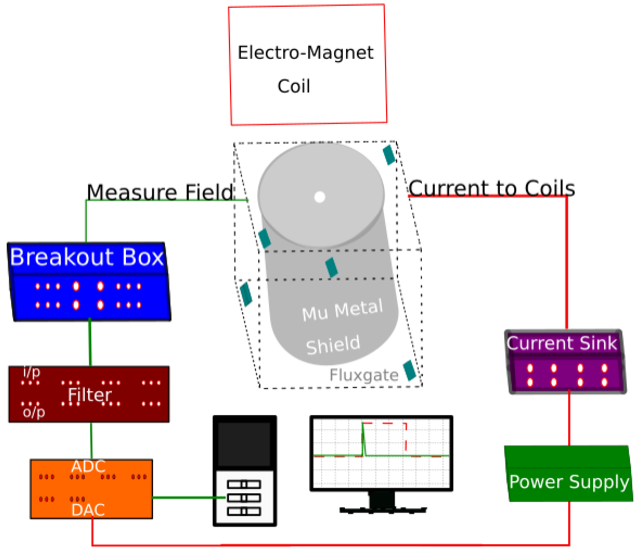
\includegraphics[width=0.4 \textwidth]{Images/exp}
%     \caption[width=0.4 \textwidth]{Schematic diagram of prototype active compensation system at University of Winnipeg . }
%     \label{fig:active shielding}
% \end{figure}
% \begin{figure}
%     \centering
%     \includegraphics[width=0.5 \textwidth]{Images/ss}
%     \caption[width=0.4 \textwidth]{PI loop in flow chart. First measurement from the fluxgates will act as set-point. Then the repeated measurements from the fluxgates are taken. For each measurement difference with the setpoint are noted. On the basis of the difference, the required amount of current for the coils surrounding the outermost layer of the shileding are determined and sent. Those coil currents generate required amount of magnteic flux to compensate for the differences.}
%     \label{fig:active shielding}
% \end{figure}
% The four layer Mu-metal cylinder enclosing the experimental area, which will be used for passive shielding has surrounded by six coils on six faces , each of having 1 mm$^2$ area. The outermost cylinder with coils surrounding it has been shown in the Fig.\ref{fig: active}. The magnetic environment is sensed by the fluxgates placed in different positions on the surface of the coils. The fluxgates that have been used are 3-axis. So, a breakout box has been built to separate each of x,y $and$ z axis in respective direction. Then, a fourth order low pass butterworh filter with cutoff frequency at 10 Hz has been built  to get rid of high frequency noise. After filtering,  the signals are transmitted to the computer via analog to digital converter (ADC) of LabJack T7 Pro for controlling via proportional integral (PI) feedback loop. 

